\documentclass[12pt,letterpaper]{report}
\usepackage[margin=1in]{geometry}
\usepackage{graphicx}
\usepackage{amsmath, amssymb}
\usepackage{bulsuthesis}  
\usepackage{setspace}
\usepackage{enumitem} 
\usepackage{booktabs,longtable,threeparttable,siunitx,tabularx,makecell}

\usepackage[style=apa,backend=biber]{biblatex}
\usepackage{csquotes}
\addbibresource{reference.bib}  
\usepackage[hidelinks]{hyperref}
\usepackage{url}

\usepackage{tikz}
\usetikzlibrary{shapes.geometric, arrows}

\tikzstyle{block} = [rectangle, draw, text width=5cm, text centered, rounded corners, minimum height=2cm]
\tikzstyle{arrow} = [thick,->,>=stealth]


\fronttitle{%
    LAKAD: A Personalized Mobile Itinerary Creator with Focus in Bulacan Tourism
} 


\author{%<-Name of the research proponents, in alphabetical order 
    Bryan Declaro 
    
    Franniel Luigi Hilario 
    
    Brian Gabriel Magbanua
    
    Richard Manansala 
}

\adviser{Aaron Paul Dela Rosa}	%<-full name of thesis adviser
\advisertitle{Mr. }	


% -------------------------------------- START -------------------------------------------------------
\begin{document}

\doublespacing

\maketitle
\setcounter{chapter}{1} % Chapter Start at 2
\chapter{Theoretical Framework}
This chapter combines significant findings from various literature and studies from tourism, exploration of the traveling salesman problem in itinerary planning, and methods for recommendation for itinerary generation. This comprehensive review will serve as the basis for the development of the LAKAD application by identifying relevant factors optimization algorithms for TSP in itinerary planning and factors to consider when creating personalized recommendation features of the system.

\section{Relevant Theories}
Key features of LAKAD rely on established theories of mathematics. This section examines the foundational theories and explains how they are used and related to the concept of itinerary optimization and personalized generation.

\subsection{Graph Theory}
Graph theory is a branch of mathematics that focuses on the study of Graphs, which are structures consisting of vertices/nodes and edges that connects the vertices on a graph. A graph $G = (V,E)$ is defined by a set of vertices $V$ and a set of edges $E$.  

The History of Graph theory is can be traced back with the problem of Königsberg Bridge in 1735. Leonhard Euler studied the problem of Königsberg Bridge and give a structure to solve the problem called Eulerian graph, which gave birth to the graph theory.  The concept of a complete graph and bipartite graph was presented by A.F Mobius in 1840. The concept of tree was established by Gaustav Kirchhoff in 1845 \parencite{Gangrade2022}. 

In this study, the concept of graph theory will be used to represent the points of interest (POI) as nodes/vertices and the distance between each connected vertex as the edges. This graphical representation is important structure for solving the Traveling Salesman Problem (TSP).

\subsection{Traveling Salesman Problem (TSP)}
This is a specific problem under the field of graph theory. According to \textcite{Pop2024}, the Traveling Salesman Problem (TSP) has been in the history of combinatorial optimization since 1930, and was properly provided a mathematical formulation by Merrill M. Flood. TSP became very popular since it is a widely investigated optimization problem, often serving as a benchmark for modern optimization algorithms. %Bresson & Laurent (2021) noted TSP as an inspired problem from the works of William Hamilton in the 19th Century, before it was formulated in 1930, and later popularized by Von Neumann in 1951.

The problem states that, given a set of cities, the salesman’s goal is to find the shortest possible route that visits each city exactly once. The TSP has many variants such as the asymmetric TSP in which the distance from point A to point B is different from point B to point A. Most real life applications of TSP are asymmetric which means ATSP is important to consider due to the presence of one way roads. It can easily be seen how the idea of TSP can be applied to itineraries. Each location of itineraries will be nodes and the distances between them are the edges. The goal of the system for the itinerary is to find the route which covers the least distance \textcite{Pop2024}.


\subsection{Orienteering Problem}
The Orienteering Problem (OP) is a routing problem that aims to maximize the total rewards collected along a route within a given travel budget \parencite{yu2022}. Similar to this, \textcite{morandi2024} explains OP as the task of planning a route for one vehicle that has to follow a travel budget. The problem is depicted as a graph where the roads have distances and the locations have points or reward values. The goal in this problem is to create a path that starts and ends at the depot, stays within the travel limit, and collects as many rewards as possible from the places visited. Similarly, it originated from a sport of the same name, where participants visit check-points with pre-determined scores, in an attempt to maximize their total score within a specific time \textcite{Lim2019}. \textcite{pvenivcka2019} described OP as a type of problem in operations research, introduced to it in 1984 by Tsiligirides. They then explained that OP is a problem that combines the combinatorial optimization problem Knapsack Problem (KP) with Traveling Salesman Problem (TSP). These two work separately as TSP, given a set of customers, seeks to find the sequence in which to visit selected customers, constrained within a budget, while also minimizing the tour path. The subset of selected customers is selected by the KP, where it maximizes the collected profit based on the selection of customers to be visited within the budget constraints. This will be used in the recommendation feature of the system where the user provides input for the time or distance constraint to generate an itinerary for the user.

% The model was first introduced by Tsiligirides and Golden et al. in the 1980s, where in the viewpoint of logistics, a vehicle must serve a set of customers, where the travel time and cost are known. The aim is to maximize the total profit of serving each customer within a time constraint \textcite{Montemanni2025}. 

\subsection{Technology Acceptance Model}
The model was first introduced by Fred Davis in 1989. It is a theoretical model that seeks to explain the attitudes in newer technologies \textcite{Aburbeian2022}. It runs on two key principles: perceived usefulness and ease of use, as these attitudes influence the users’ actual usage or rejection of the technology. This model will provide insights to how likely to adopt the existence of the LAKAD application. TAM will be used to assess the capability of the proposed system through the cooperation of its end users.

\subsection{Software Product Assessment Framework (ISO 25010)}
The ISO 25010 is an international standard for assessing and evaluating the quality of systems and software \textcite{Peters2020}. This framework will be used in the study’s evaluation of the proposed system to ensure the system will meet the high-quality standards.


\section{Review of Related Literatures and Studies}
This section presents studies relevant to the development of the proposed itinerary planner. It covers works on Bulacan tourism, optimization techniques for the Traveling Salesman Problem (TSP), and related approaches in itinerary planning. By reviewing these studies, the foundation for the system is established and the choice of African Buffalo Optimization (ABO) as the core algorithm is justified.

\subsection{Tourism in Bulacan}
The study of \textcite{Canet2024P} found that tourism development in Bulacan is highly influenced by accessibility, infrastructure, promotion, and the preservation of cultural and natural heritage. While Bulacan shows great potential as a tourist destination because of its rich history and heritage, the issues such as weak promotion, limited facilities, and transportation continue to limit its growth. A study by \textcite{Canet2025S}, investigates why some historical and cultural destinations in Bulacan remain neglected despite the province’s rich heritage. Using a mixed method design, they combine surveys and interviews to capture both statistical data from tourists and tourism officers. The survey results showed that most visitors were young ranging from 19 to 29. Most of the respondents are women and most of the tourists came from within Bulacan itself. The findings of the study showed that popular landmarks like Barasoain Church and the Basilica Minore de Immaculada Conception, both in Malolos City, attract the most visitors. On the other hand, attractions in other municipalities such as Meyto Shrine in Calumpit and Francisco Balagtas Museum in Balagtas, showed lower visitations. This imbalance reflects the uneven promotion of Bulacan’s cultural sites.

This uneven promotion aligns with the findings of \textcite{Canet2024P} that one of the issues is the weak promotion. Fortunately, Canet and Sunpongco examined the promotional strategies used by tourism offices and found that online promotions, social media campaigns, and partnership with bloggers and vloggers were the most effective methods of engaging younger audiences. While traditional approaches such as brochures, festivals and community-driven activities still play a role, digital strategies are better suited for Gen Z and millennial demographic.  They emphasized the importance of collaboration among local government units, schools, communities, and tourism stakeholders to ensure consistent promotion and sustainable tourism development.  

The local government of Bulacan has also recognized the importance of tourism in the province. In 2023, the Provincial Government of Bulacan launched the Bulacan Heritage Pass a tourism initiative that focuses on local culture, heritage conservation, and community engagement. The Pass consists of twenty historical and cultural landmarks in the province. The landmarks include Barasoain Church, Casa Real de Malolos, the Malolos Cathedral, and the historic train stations in Guiguinto and Meycauayan, offering a structured route and incentives for completion \textcite{Velasco2023}. While the Heritage Pass strengthens heritage preservation and promotional efforts, it does not provide optimized travel sequencing for visitors, leaving tourists to plan routes on their own. This gap underscores the need for systems that not only identify attractions but also generate efficient itineraries tailored to tourists’ time and travel constraints.

Digital strategies also play a critical role in Bulacan’s tourism promotion, \textcite{Santos2023}, studied how social media content is disseminated to the users. They surveyed a total of 100 respondents (50 working staff + 50 tourists) in San Rafael, Bulacan and found that 57 percent agreed that social media helped them determine their next choice of destination and 61 percent agreed that social media is a good strategy to make more tourist locations known to people. In line with this, \textcite{DelaCruz2022} also surveyed 100 tourists that visited Dona Remedios Trinidad, Bulacan to determine the effectiveness of using social media in promoting a tourist destination and asked questions ranging from how social media influences traveler’s decisions to the problems faced by tourists when using social media as a guide for tourism. They found that most travelers agreed that social media does influence the choice of  destination of travelers. While problems reported by tourists is the spread of false or misleading information, different expectations, and inaccurate photos / videos to different tourist destinations. Clearly, the importance and role of social media in making tourist locations well-known is irreplaceable but is also prone to misleading information, highlighting the need for verified and curated information of tourist attractions in Bulacan.

\subsection{Existing Optimization Techniques for TSP}
Traveling Salesman Problem (TSP) has many ways to solve it using different algorithms, one of those is the exact method. According to \textcite{Violina2021}, exact methods such as Brute Force and Branch and Bound algorithms are used to solve the TSP. The brute-force method involves trying each possibility one at a time until all of them have been explored, comparing the outcomes, and selecting the smallest one. When applying brute force to the TSP, the outcome is be optimal but less effective. This is because every possible combination must be tested before obtaining the best results. Applying this technique results in O(n!), where n is the number of cities that need to be traversed. Even with just 20 cities, a solution like this is not feasible.

In contrast, the Branch and Bound (BB) algorithm is a technique for methodically searching the solution space. In this case, a status space tree is used to arrange the solution space. This algorithm uses a broad search scheme, often known as Breadth First Search (BFS), to build a status space tree. However, the expanded node is determined by the node with the lowest "cost" value among the other live nodes rather than the sequence of generation. Although exact algorithms like Brute Force and Branch and Bound provide optimal solutions, they are restricted by exponentially growing time complexity as the number of vertices increases. %Hougardy and Zhong (2018) showed that Concorde exact solvers for the Traveling Salesman Problem take days to compute for instances with only a few hundred cities. This highlights the limitation of exact methods for mobile operation or real-time flight planning, where efficiency and expediency are essential.

Heuristic approaches, particularly nature-inspired metaheuristic algorithms \textcite{Sabery2023}, offer computationally efficient solutions for real-world optimization problems. Generally, metaheuristic algorithms begin with an initial solution and follow a set of heuristic principles to explore the search space and iteratively improve it. These guidelines help the algorithm avoid local optima and locate globally optimal or nearly optimal solutions by directing the search process toward promising areas of the search space.

In line with this, \textcite{BarbCiorbea2023} compared an exact method, Mixed Integer Linear Programming (MILP), with a heuristic approach, Ant Colony Optimization (ACO), for solving the Traveling Salesman Problem with time window constraints. In the experiment, the MILP formulation with 100 cities generated more than 1000 variables, while the heuristic approach was limited to 15 ants. Results showed that MILP required more than 500 seconds to obtain the solution, whereas ACO was able to produce results in about 100 seconds. The exact approach is advantageous because it guarantees the best solution; however, its runtime becomes very high as the number of cities increases.

For larger instances, the heuristic approach produced solutions much more quickly, although without the guarantee of global optimality. Despite this, both algorithms were able to achieve the best result in the tested scenario. Moreover, the heuristic demonstrated an additional advantage by aiming to minimize waiting duration at nodes when waiting could not be avoided. These findings emphasize that while exact methods provide precision, heuristic methods like ACO are better suited for larger and more time-sensitive problems \parencite{BarbCiorbea2023}. This demonstrates that while exact methods are strictly optimal with respect to accuracy, their exponentially growing time complexity renders them impractical to apply to large-scale or time-constrained situations. 

The goal of most heuristic algorithms is to find an optimal path to an instance of the traveling salesman problem. For instance, the study of \textcite{Wu2020} applied the Aggloremative Greedy Brain Storm Optimization (AG-BSO) in solving instances of the traveling salesman problem. This algorithm is a variant of what is called the Brain Storm Optimization framework (BSO), a method that addresses the computational challenges posed by TSP using the concepts modeled after human brainstorming. They compared AG-BSO with traditional metaheuristic strategies like Genetic Algorithm (GA), Particle Swarm Optimization (PSO), Simulated Annealing (SA), and even Ant Colony Optimization (ACO). The results found AG-BSO achieved greater solution accuracy and better robustness producing less standard deviation, which for most instances is less than 1 percent, compared to traditional algorithms.

The increased robustness was also found in the study of \textcite{Hossain2024} where they compared new optimization algorithms against old optimization algorithms for solving the Traveling Salesman Problem and concluded that the new algorithms demonstrated greater effectiveness than the old algorithms in medium-scale instances. The new algorithms used in the study which are the Artificial Bee Colony (ABC), Grey Wolf Optimization (GWO), and the Salp Swarm Algorithm (SSA) performed with a lot less standard deviation compared to the classic algorithms such as the Genetic Algorithm (GA), Ant Colony Optimization (ACO), and Simulated Annealing (SA). This means that on average, the three newer algorithms produced more consistent results than the classic three. However, they also stated that although newer algorithms produced better outputs, traditional algorithms such as GA and ACO remained to demonstrate strengths for specific instances. The findings of \textcite{Odili2021} also aligns with it as they studied some complex hybrid models’ performance such as Cooperative Genetic Ant System (CGAS), Max-Min Ant System (MMAS), and Model-Induced Max-Min Ant Colony Optimization (MIMM-ACO) were found to have an error of 2.56 percent only with MIMM-ACO having 0 percent error and accurately solving all instances given in the study.

However, this great performance output from these algorithms comes at the cost of greater computation time. The AG-BSO algorithm from the study of \textcite{Wu2020} took a whole 9.05 seconds to solve a small vertex TSP instance. This performance to computation time discrepancy also aligns in the comparative study of \textcite{Hossain2024} where ABC took an average of 4 seconds, 3 seconds for SSA, and 7 seconds for GWO when solving small vertex TSP instances. While an average of 15.5 seconds for MIMM-ACO, 32.83 seconds for MMAS and 52.02 seconds for CGAS was observed by \textcite{Odili2021} for solving the given instances in their comparative study. While newer and complex algorithms outperform traditional ones in accuracy and robustness, their higher computation times may pose challenges for resource-constrained environments such as mobile devices. 

While some algorithms found focus on the accuracy of finding the most optimized route, there are still approaches that not only prioritizes optimal routing but also the speed at which it can be obtained. This is demonstrated in the study of \textcite{Hossain2024} where they compared new optimization algorithms against old optimization algorithms for solving the Traveling Salesman Problem. The new algorithms Artificial Bee Colony (ABC), Grey Wolf Optimization (GWO), and Salp Swarm Algorithm (SSA) are compared to traditional metaheuristic algorithms like Genetic Algorithm (GA), Ant Colony Optimization (ACO), and Simulated Annealing (SA). The new algorithms show promising results in quickly finding a quality optimized route for medium-scale instances of 200 - 500 vertices, as compared and confirmed by a t-test against GA, SA, and ACO. On the other hand, a different comparative study of \textcite{Wadi2025} highlighted the capability of ACO and Particle Swarm Optimization (PSO) to provide a fast execution speed with minimal solution quality reduction, albeit PSO being parameter-sensitive. They also examined another swarm-based approach in the form of  Elephant Herding Optimization (EHO), which consistently outperformed both ACO and PSO by achieving lower optimal costs while maintaining short execution times. Their study demonstrated the practicality of the swarm-based approaches in large-scale instances, over exact methods.

There are also algorithms that focus on faster execution time at the cost of less solution quality to the route planning. These fast algorithms, however, are most suitable for hardware-related limitations such as processing power in mobile devices. The study of \textcite{Odili2021}, comparing five metaheuristic algorithms and one heuristic algorithm to solve the TSP using 15 instances from TSPLIB, shows that the metaheuristic algorithm, African Buffalo Optimization (ABO), a swarm-inspired algorithm from the ability of buffalo herds to organize, had an accuracy of 98.6 percent and is the fastest to complete all instances with only a total computation cost of 20.58s, 3 times faster than the above-mentioned MIMM-ACO. Thus, their study concluded that ABO is the better algorithm of all six compared in terms of efficiency. PSO has also been shown to perform well in terms of runtime as \textcite{Wadi2025} found that it provided faster solutions compared to ACO across a variety of problem sizes, although PSO was observed to be sensitive to parameter configurations. Simulated Annealing, being a traditional approach, also proved its value in great runtimes as \textcite{Hossain2024} noted its performance in small-scale datasets with 14 - 52 vertices. Overall, PSO excels in rapid convergence across varying problem sizes, SA remains an effective option for small-scale applications, and ABO provides the best balance of accuracy and speed. %(Odili et al., 2021; Wadi & Umar, 2025; Hossain & Acar, 2024).

However, it is important to note that many of these algorithms have been tested under different experimental settings and datasets. Some studies evaluate multiple algorithms on the same benchmark, such as ABO against other metaheuristics in the study of \textcite{Odili2021}, or ABC, GWO, SSA, GA, ACO, and SA in the study of \textcite{Hossain2024}, or ACO, PSO, and EHO in \textcite{Wadi2025}. Although, ACO is mentioned twice, it is important to note that they are tested under different experimental conditions, which makes direct comparison across studies difficult. As a result, the performance of an algorithm such as ACO may vary between studies depending on the dataset and evaluation criteria.

Despite these differences, the literature consistently highlights African Buffalo Optimization (ABO) as a balanced approach in terms of accuracy and computational speed. This study does not claim that ABO is universally superior, rather it is identified as the most suitable choice for the proposed system due to its efficiency in resource-constrained environments like mobile devices. Supporting this, \textcite{Odili2020Swarm} demonstrated that ABO achieved better or near-optimal solutions across multiple TSP benchmarks, with lower margins of error compared to other swarm-based methods. Similarly, \textcite{Algani2023} reported that ABO outperformed both the Lin-Kernighan algorithm and Honey Bee Mating Optimization, attaining up to 99.5 percent accuracy while requiring significantly less computation time for asymmetric TSP. These findings highlight ABO’s practicality for mobile applications, where both speed and efficiency are critical.


\subsection{Tourism Recommender Systems}

% Overview
Tourism is an important aspect of society, as it enables people to explore different places, cultures, and experiences while also contributing to economic and social development. Organizing trips, whether to a destination or multiple destinations, usually requires a lot of time and effort. \textcite{kedkaew2024} note that while acquiring travel information for planning a trip is important, the experience is not without challenges, for acquiring and evaluating travel plans is a lot of work. In response to this challenge, \textcite{alrasheed2020} describe tourism recommender systems as tools integrated in travel and tourism applications that enhance service quality by filtering vast amounts of information on the web and customizing it to travelers’ particular needs. Such systems help people find destinations matching their needs and constraints, for example, financial need or travelling dates, while also considering contextual factors like weather and safety. In essence, tourism recommender systems are decision-support tools that simplify the destination planning and improve travel experience.

% General Recommendation System
With the ever-increasing data available online through social media, personalized recommender systems have been able to provide better recommendations and have become more relevant in our lives, making it easier to discover new things in life \parencite{Li2023}. 

% Collaborative Filtering
One popular recommendation method is through Collaborative Filtering (CF). This method is used to predict a user’s preferences or opinions by using the collective information of other users of the system. It basically analyzes the similarity between user’s preferences and provides a recommendation that way \parencite{Li2023,Widayanti2023}. However, this method is severely set back by the “cold start” problem where it requires a large enough data of users and their interaction to generate recommendations. Thus, this method is not applicable for the proposed system as no user to user interaction is planned, and the system is a standalone mobile application where the algorithms run on the device locally. 

% Content-Based Filtering
Another popular recommendation method is the Content-based Filtering (CBF). It uses a feature list of item and compare it with items preferred by a specific user previously. The items that match in similarity are recommended to the user. CBF works by storing user profile based on item features which are most commonly preferred by the user. These features are used to map the similarity of one item with other by similarity equation. Then, it compares each item’s features with the user profile and recommend it based on the degree of similarity. Unlike CF, it does not require any feedback from the user \parencite{Raghuwanshi2019}. However, just like CF, it is also prone to the “cold start” problem especially for new users. Additionally, CBF doesn't have much control over route-level constraints like travel time, distance and budget. 

Due to the shortcomings of CF and CBF and since the proposed system is standalone mobile application with no external server, An algorithmic approach is the desired approach for TRS. One algorithmic approach is based on Orienteering Problem (OP). According to \textcite{Lim2019} Tour recommendation has its roots in the OP and similar variants where a key
feature is that they do not incorporate any personalization for individual users. 

A study by \textcite{Yochum2020} proposed an Adaptive Genetic Algorithm with dynamic crossover and mutation probabilities (AGAM) to handle personalized multi-objective itinerary planning. Their approach integrates mandatory POIs, popularity ratings, visit duration, travel time, and costs into a weighted fitness function. By using data from platforms like TripAdvisor, GoogleMaps, and Flickr, AGAM adapts during evolution to avoid stagnation and produce diverse solutions. They tested the model with a dataset for six cities namely Budapest, Edinburgh, Toronto, Glasgow, Perth, and Osaka. AGAM was compared against two baseline heuristics, MaxN a greedy approach that prioritizes the maximum number of POIs, and MaxP also a greedy approach that prioritizes POIs with the highest rating. The results show that while MaxN and MaxP performed better at including mandatory POIs, AGAM generated richer itineraries with higher-rated POIs. AGAM shows more effective use of time budgets, and improved user enjoyment, but at the expense of higher cost and fewer mandatory POIs. This study shows that algorithmic approach can provide personalized itinerary for tourists. 

Another study by \textcite{Tenemaza2020}, proposes a mobile recommender system that addresses the Tourist Trip Design Problem (TTDP), modeled as a Time-Dependent Orienteering Problem with Time Windows (TDOPTW). The aim was to build a system that not only recommends tourists itineraries but also optimizes them in real time while considering Tourist’s personal interest, POI constraints (opening hours, time of visit, travel time), and Contextual factors such as lunch times and location. Their approach combines k-means clustering to organize POIs based on user interests and available days with Genetic Algorithm enhanced with parameterized fitness function to include any element of the context to create an optimized recommendation. To test the power of their recommender system, they create a mobile application that uses their algorithm. Evaluation with 131 tourists demonstrated that accuracy and diversity of recommendations strongly influenced user satisfactions. Retrieval metrics such as precision and recall confirmed the system’s ability to balance tourist preferences with contextual constraints. 

Together, these studies show a similar research direction in tourism itinerary optimization with metaheuristics. The AGAM framework by \textcite{Yochum2020} highlights adaptability through genetic algorithms and diverse real world data sources to produce personalized itineraries. On the other hand, the TD-OPTW approach of \textcite{Tenemaza2020} focuses on contextual constraints, ensuring that the generated itineraries are not only optimized but also feasible in practice. While AGAM prioritizes richer and higher rated itineraries even at the cost of efficiency, \textcite{Tenemaza2020} balances user interest with practical constraints. These results indicate that algorithmic approach can provide personalization as opposed to \textcite{Lim2019}.  All in all, these studies show the effectiveness of metaheuristic methods in tourist applications, demonstrating that algorithmic strategies can significantly improve the quality, adaptability, and satisfaction of itinerary recommendations. 

% Orienteering Problem Approach
% Orienteering Problem is a class of routing problems that aims to maximize profit obtained through a single determined route over a time period, which also maximizes the number of visited customers \parencite{yu2022}. Similar to this, \textcite{morandi2024} explains OP as the task of planning a route for one vehicle that has to follow a travel budget. The problem is depicted as a graph where the roads have distances and the locations have points or reward values. The goal in this problem is to create a path that starts and ends at the depot, stays within the travel limit, and collects as many rewards as possible from the places visited \textcite{pvenivcka2019} described OP as a type of problem in operations research, introduced to it in 1984 by Tsiligirides. They then explained that OP is a problem that combines the combinatorial optimization problem Knapsack Problem (KP) with Traveling Salesman Problem (TSP). These two work separately as TSP, given a set of customers, seeks to find the sequence in which to visit selected customers, constrained within a budget, while also minimizing the tour path. The subset of selected customers is selected by the KP, where it maximizes the collected profit based on the selection of customers to be visited within the budget constraints.

% \textcite{yu2022} extends OP to Team Orienteering Problem (TOP), which is a variant of the problem where multiple vehicles maximize the collected profit through each of their determined routes, essentially situating OP into a multi-objective problem by implementing a multi-route planning variable. Related to this, \textcite{Yochum2020} proposed an Adaptive Genetic Algorithm with dynamic crossover and mutation probabilities (AGAM) to handle personalized multi-objective itinerary planning. Their approach integrates mandatory POIs, popularity ratings, visit duration, travel time, and costs into a weighted fitness function. By using data from platforms like TripAdvisor, GoogleMaps, and Flickr, AGAM adapts during evolution to avoid stagnation and produce diverse solutions. They tested the model with a dataset for six cities namely Budapest, Edinburgh, Toronto, Glasgow, Perth, and Osaka. AGAM was compared against two baseline heuristics, MaxN a greedy approach that prioritizes the maximum number of POIs, and MaxP also a greedy approach that prioritizes POIs with the highest rating. The results show that while MaxN and MaxP performed better at including mandatory POIs, AGAM generated richer itineraries with higher-rated POIs. AGAM shows more effective use of time budgets, and improved user enjoyment, but at the expense of higher cost and fewer mandatory POIs.


\section{Review of Related Systems}

This section presents different related systems that feature such as: itinerary optimization, where in a group of locations is selected and the order of visitation becomes an output; and personalized itinerary recommendation, where based on the user’s preferences and other factors, an itinerary is generated.

\subsection{Trippit: An Optimal Itinerary Generator}

Trippit by \textcite{Nguyen2020} addresses a fundamental problem in itinerary planning which is the optimization of the itinerary itself which is a fundamental limitation of Google Maps. Although Google Maps supports multiple stops, it leaves the sequencing to the user and often resulting in inefficient trip planning. Manual planning takes time and significant effort to optimize in terms of total distance traveled and how long each location to visit for. The study also stressed the fact that most travelers would often switch between Google Maps and Yelp for planning itinerary. The system eliminates the difficulty in travel planning which makes vacation trips more time efficient and enjoyable to travelers. 
	
The system was developed using the Waterfall method where each design phase is completed first before beginning the next. An android application was developed using React Native library and called network APIs such as the Google Places API and Foursquare Places API to calculate the optimized itinerary provided by the user. Users can input point of interests (POI) in which the application then retrieves the information from the respective APIs and calculates and outputs the optimized tour based on a greedy algorithm. Their system also calculates the best time to visit each input.
	
Trippit underwent several testing phases: primary testing, where they compared the results of the system to a known small list of itineraries; unit and integration testing, where they tested the logic and the correctness of the user interface; and alpha testing, with 10 users and was validated using a user satisfaction survey, in which most of the alpha users were satisfied with the resulting itinerary.  However, through the selection of the algorithm  and device came its limitation, which is that the application can only process up to 12 points of interest (POI). Its evaluation is also a concern as it didn’t use any standard evaluation methods like ISO/IEC 25010:2023 standard or the Technology Acceptance Model (TAM). Although a small prototype, Trippit can be considered a good enough system as it was able to produce good itineraries with a simple smartphone application without the use of advanced tools like Google OR.



\subsection{Optimization of Tourism Destination Recommendations in Batang Regency Using Content-based Filtering}

\textcite{Yulfihani2024} created a tourism recommendation system for Batang Regency in Indonesia. They applied Content-Based Filtering (CBF) for their recommendation system, using tourist preferences as their data source. Tourists interact with the system by adding destinations to a wishlist. The system then uses the wishlist to learn the tourist’s preferences. The recommender factors category similarity where it compares the categories of wishlist items like nature, culture, culinary, and leisure; and location similarity by calculating the distance between destinations using the Haversine formula, which finds the shortest distance between two points on Earth using latitude and longitude.  The total similarity then calculated with 70 percent category similarity and 30 percent location similarity. The system ranks all available attractions by their total similarity score and the top 10 destinations are recommended to the tourist. The system was tested in different scenarios such as single item in wishlist, multiple items from same category with same/different locations, and multiple items from mixed categories. They use precision, recall, and F1 score as a metric for the system. 

The system was designed with a three-tier architecture that includes Backend, Web Admin Panel, and Mobile Application. The backend was built using Laravel (PHP framework) and MySQL, it acts as the hub for all operations including user authentication, processing recommendations using the CBF algorithm, and managing communication between the mobile app, admin panel, and database. The Web admin panel is for administrators and also developed using Laravel, it enables admins to manage tourist destinations, categories (nature, culture, culinary, etc.). Any changes made in the admin panel updates the backend database which instantly reflects to the mobile apps. The Mobile application was developed using Android Studio and Kotlin, it connects the backend using RESTful APIs via Retrofit. The app provides tourists with Login/registration, wishlist management, personalized recommendation based on wishlist and CBF algorithm, viewing details of attractions, and Filtering by categories and proximity.

The system provides highly accurate and relevant recommendations for tourists, especially in simple preference scenarios. The Content-based filtering approach worked well for aligning recommendations with tourists interests, and achieving a very high F1 score of 0.965. However, performance dropped slightly in complex scenarios like when the wishlist items mixed with different categories and locations. The Authors recommend future improvements such as expanding the dataset, using hybrid models (CBF + collaborative filtering), and adding user feedback mechanisms to further refine recommendations. 

However, their study is solely focused on the recommendation aspect of the system, and not on the itinerary optimization. While the system can recommend destinations based on user preferences, it does not optimize the sequence of visits or consider travel constraints like time and distance. Additionally, they didn’t include an evaluation for the system like  ISO/IEC 25010:2023 standard or the Technology Acceptance Model (TAM), only the evaluation for the Content-based filtering was provided.


\subsection{Visit Planner: A Personalized Mobile Trip Design Application based on a Hybrid Recommendation Model}

Visit Planner (ViP) a mobile application prototype developed by \textcite{papadakis2024}. It offers personalized recommendations for an itinerary based on user preference which are either explicitly collected by the application or assessed through the user’s behavior within it. ViP utilizes an Expectation Maximization method to offer the user an itinerary that tailors to their satisfactory needs while taking into consideration time and spatial constraints that concern both the user and the destination. The application currently focuses on the city of Agios Nikolaos in Crete. The system requires a user to create a secured profile in a registration process, wherein demographic information and essential data for the algorithm is collected. After this registration process, the user is also asked to specify their preferences in three different ways of their choice, one is by rating categories of POI, another choice is by stating if they like or dislike the category, and another one is by selecting their most preferred category. These categories are carefully specified by analyzing responses collected from 150 visiting tourists, in addition to local and expert knowledge in Agios Nikolaos.

The architecture of the system consists of main components like the front-end User Interface, back-end database, the middleware for processing the information, the recommendation components, and the itinerary creation components. The front-end of the application is an android app available in Google Play. The back-end is composed of MariaDB databases for the purpose of storing necessary information of users and POIs for smooth operations and functionalities. The middleware, built upon the basis of Spring Boot Framework aims to process the controlling flow between the system components and perform the functionalities. It works by receiving queries from the front-end, and then sending those to the recommendation algorithms. The recommendation and itinerary creation components comprises four several recommendation algorithms to tender the needs of the user, where each user is assigned a different algorithm for their cases in performance evaluation wise. ViP integrates multiple, novel recommender algorithms which can adapt to different user profiles. 

The algorithms include model-based collaborative filtering that uses synthetic coordinate based system for recommendations (SCoR), hierarchical content-based similarity measures, a hybrid content-based recommendation using Weighted Extended Jaccard approach combined with the second one, and Bayesian recommender algorithm. Any of these algorithms is applied to generate personalized POI suggestions. And once candidate POIs are retrieved, an expectation-maximization-based itinerary creation component sequences them into a feasible route by maximizing user satisfaction function constrained under temporal and spatial factors.


\subsection{I-AIR: Intention-aware travel itinerary recommendation via multi-signal fusion and spatiotemporal constraints}

\textcite{Cui2025} developed I-AIR (Intention-Aware Itinerary Recommendation), a system based on deep learning that aimed to generate personalized and practical traveling itineraries. The two primary components of the system are an Itinerary Construction Policy, which organizes selected Points of Interest (POIs) into a logical and sequential trip, and an Intention-Aware POI Scoring Model, which assesses the relevance of possible POIs based on user preference and contextual cues. To model user preferences, I-AIR applied a Transformer-based sequential encoder that identified time patterns from check-in history, an explicit feedback encoder that synthesized long-term preferences from ratings and likes, and a Graph Convolutional Network (GCN) that represented POI relationships through co-visitation patterns. These components were integrated via a multi-signal fusion layer to generate customized POI relevance scores. In optimizing the route, the system applied a greedy algorithm that picked the top-scoring viable POI at each step while removing possibilities that violate prohibitions such as travel time, wait time, business hours, and total time budget. The model was trained using a combination of next-POI prediction and explicit feedback reconstruction on datasets including user trajectories, ratings, dwell times, and POI attributes.
 
During evaluation, the system was tested on eight real-word datasets, including four each of theme parks and city tourism. These datasets included detailed information such as user check-in records, wait times at attractions, and tourists' reviews, and provided implicit and explicit feedback signals. The evaluation measures applied were precision, recall, and F1-scores, and comparative baseline systems included were Greedy-Popular (GPop), Greedy-Near (GNear), PersQ, EffiTourRec, DCC-PersIRE, BERT-Trip, and DLIR. Results showed that I-AIR outperformed the other systems significantly across all datasets, with higher precision in both theme park and city tourism scenarios.

\section{Synthesis of the Review}

The reviewed theories and literature establish the foundations and identify the gaps that this study aims to address. Graph Theory, the Traveling Salesman Problem (TSP), and the Orienteering Problem provide the mathematical framework for route optimization, while models such as the Technology Acceptance Model (TAM) and ISO 25010 serve as evaluative guides for usability and system quality. Prior research highlights the limitations of exact algorithms in solving large-scale routing problems, particularly in mobile environments with limited computational resources. This has led to the rise of heuristic and metaheuristic approaches. Among these, African Buffalo Optimization (ABO) emerges as a promising solution due to its demonstrated balance between accuracy and efficiency, outperforming or matching other metaheuristics such as Genetic Algorithms, Ant Colony Optimization, and Particle Swarm Optimization, while requiring fewer resources. These characteristics make ABO well-suited for itinerary planning on mobile devices.

In the context of tourism, studies reveal that Bulacan’s cultural and historical richness remains underutilized due to weak promotion and uneven visitation across sites \textcite{Canet2025S}. While initiatives such as the Bulacan Heritage Pass \textcite{Velasco2023} showcase heritage landmarks and encourage structured visits, they do not provide optimized sequencing of destinations. Likewise, existing tourism applications and mapping systems offer navigation but lack integrated route optimization. Social media, although influential in promoting destinations, presents risks of misinformation and lacks curated, reliable guidance for tourists.

Taken together, these findings underscore the need for a system that not only promotes Bulacan’s tourist sites but also generates optimized itineraries tailored to visitor preferences, time, and travel constraints. This study addresses that gap by developing a mobile-based itinerary recommender system powered by ABO. By bridging theoretical optimization methods with the practical needs of local tourism, the system contributes both to computational research and to Bulacan’s cultural tourism development.


\section{Conceptual Framework}
This section explains the key inputs, processes, and outcomes in development of the study using an Input-Process-Output (IPO) model.

\begin{figure}[h]
\centering
\caption{Input-Process-Output Model of the Study}
\label{IPO}
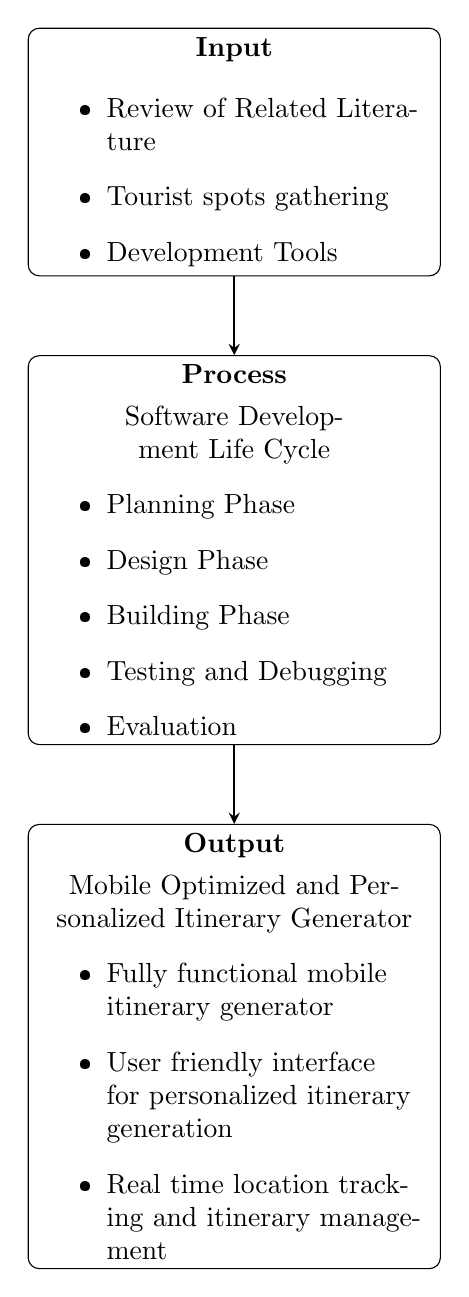
\begin{tikzpicture}[node distance=1cm]

% Nodes
\node (input) [block, anchor=north] at (0,0) {
    \textbf{Input} \\[3pt]
    \begin{itemize}
        \item Review of Related Literature
        \item Tourist spots gathering
        \item Development Tools
    \end{itemize}
};

\node (process) [block, anchor=north] at ([yshift=-1cm]input.south) {
    \textbf{Process} \\[3pt]
    Software Development Life Cycle
    \begin{itemize}
        \item Planning Phase
        \item Design Phase
        \item Building Phase
        \item Testing and Debugging
        \item Evaluation
    \end{itemize}
};

\node (output) [block, anchor=north] at ([yshift=-1cm]process.south) {
    \textbf{Output} \\[3pt]
    Mobile Optimized and Personalized Itinerary Generator
    \begin{itemize}
        \item Fully functional mobile itinerary generator
        \item User friendly interface for personalized itinerary generation
        \item Real time location tracking and itinerary management
    \end{itemize}
};


% Arrows
\draw [arrow] (input) -- (process);
\draw [arrow] (process) -- (output);

\end{tikzpicture}
\end{figure}

\subsection{Input}
The input contains the review of the methods used by related studies and systems, which will be used as foundation in the study. These methods consist of different algorithms used for solving the traveling salesman problem and selecting which algorithm is the most applicable in the mobile platform as well as which recommendation model is a fit for itinerary recommendation. The second input is the gathering of tourist spot locations or point of interests (POI). These POIs are locations in Bulacan which can be considered as tourist attractions. These will be gathered from and verified by the Provincial History, Arts, Culture, and Tourism Office (PHACTO) to assess the correctness of the POIs included in the system. Development tools refer to the hardware and software tools that will be used to actually develop the application. These include operating systems such as Windows or Ubuntu, integrated development environments (IDE) such as Visual Studio or Android Studio, and design pieces of software like Figma or Adobe Illustrator.

\subsection{Process}
The AGILE methodology will be used in the software development of LAKAD, specifically the Kanban method. Kanban method is  a  visual  process  management  system that can manage knowledge and work by considering the Just In Time (JIT) delivery approach \textcite{Alaidaros2021}. The first phase of the development will be planning and analyzing the different requirements of the system such as flow charts, entity relationship diagrams, and use cases. Afterwards, mockup user interface will be made to fully outline the look and feel of the application. Building phase will be the actual development of the core features of the application and testing and debugging will refer to the testing of the correctness of the core features’ implementation. The power of AGILE methodology will be used to iteratively cycle between building phase and testing to evaluation by users and professionals to quickly enhance features and get immediate feedback. The system will go through rigorous evaluation by professionals through ISO 25010 and through TAM by its intended users.

\subsection{Output}
The expected output of this study is a fully functional mobile itinerary recommendation and optimization system in the scope of Bulacan. LAKAD application will be able to optimize the route to be taken for the user's itinerary as well as recommend personalized itineraries that may interest the user.

\printbibliography[heading=bibintoc,title={REFERENCES}] %<-start the bibliography
\end{document}